\documentclass[a4paper,12pt]{article}
\usepackage{graphicx}
\usepackage{geometry}
\usepackage{algorithm}
\usepackage{algpseudocode}
\usepackage[parfill]{parskip}
\usepackage[czech]{babel}
\usepackage[utf8]{inputenc}
\usepackage{fancyhdr}
\usepackage{enumitem}
\usepackage{gensymb}
\usepackage{amsmath, amssymb, amsfonts}
\usepackage{graphicx, caption}
\graphicspath{ {./images/} }
\geometry{
total={170mm,257mm},
 left=20mm,
 top=20mm
 }
 
\title{Technická zpráva úkol č. 4: Energetické spliny} 
\author{Miroslav Hrubeš, Lucie Peterková} 
\date{Praha 2023} 
\usepackage{graphicx} % Required for inserting images

\frenchspacing
\begin{document}
    \maketitle
    \newpage
    % Zadání
    \section{Zadání}
    \textbf{Úloha č. 4: Energetické spliny}\\
    S využitím generalizačního operátoru Partial Modification realizujte odsun a částečnou změnu tvaru jednoho blízkého prvku vůči blízkému pevnému prvku (bariéře), tak aby v generalizované mapě nedošlo k jejich grafickému konfliktu. Hodnotu minimální vzdálenosti prvků d volte v závislosti na měřítkovém čísle mapy (např. 1 mm v mapě). Pro implementaci použijte metodu energetických splinů.
    
    Jako vstupní data použijte existující kartografická data (např. silniční síť, železniční síť, vodstvo), která budou načtena ze dvou textových souborů ve vašem zvoleném formátu.
    
    Grafické rozhraní realizujte s využitím frameworku QT, výsledky generalizačních operací vizualizujte. Porovnejte dosažené výsledky s ruční generalizací prováděnou kartografickým expertem.

    \section{Bonusové úlohy}
    Nebyly řešeny žádné bonusové úlohy.

    \newpage
    \section{Popis a rozbor problému}
    \subsection{Energetické spliny}
    Energetické spliny jsou v digitální kartografii využívány k transformaci původních dat do nových, generalizovaných dat. Cílem je minimalizovat deformace v původních datech, zatímco zajišťujeme, aby výsledná generalizovaná mapa měla předem stanovenou minimální vzdálenost mezi prvky.

    Tento problém vzniká při generalizaci digitálních map, kdy je potřeba zmenšit měřítko mapy, a tedy zobecnit jednotlivé prvky, aby mapa byla stále čitelná. Zároveň je ale nutné zachovat obecnou podobu původních dat a minimalizovat deformace, které mohou nastat při změně velikosti prvku.

    Tato metoda měří míru ohybu nebo zakřivení křivky pomocí energie. Cílem je vytvořit co nejhladší křivku, která přesně reprezentuje datové body.

    Pro úpravu funkce energie se využívá operátoru částečné modifikace, který upravuje tuto funkci v lokální oblasti kolem vybraného bodu, aby se výsledný energetický spline lépe přizpůsobil lokální geometrii modelované křivky. Na tvar výsledné křivky má vliv vnitřní ($E_i$) a vnější ($E_e$) energie splinu. Energetický model pro křivku L o délce l lze zapsat jako
    \begin{align*}
    E(d) &= \int_0^l E_i(s) , ds + \int_0^l E_e(s) , ds
    \end{align*}
    kde ds představuje parametrické vyjádření křivky.

    Vnitřní energie ($E_i$) splinu definovaná vztahem ovlivňuje průběh splinu a jeho tvar. První člen měří vzdálenost splinu od původního elementu, druhý napětí (elasticitu) splinu a poslední tuhost (křivost) splinu. Vliv těchto faktorů je modelován s využitím trojice parametrů $\alpha(s)$, $\beta(s)$, $\gamma(s) \in \mathbb{R}^+$. Spline tedy může více či méně sledovat původní prvek.

    Vnější energie ($E_e$) popisuje deformaci splinu způsobenou vnějšími silami. Energetická funkce, která popisuje silový model, může mít mnoho forem. Z matematického hlediska by měla být spojitá v bodě, diferencovatelná a mít jednoduchý průběh bez zbytečných oscilací. Její minimum je blízko svislé osy bufferu. Rozhodující faktory ovlivňující míru deformace představují gradient (strmost) a omezenost funkce shora. Čím větší jsou funkční hodnoty, tím silnější je jejich vliv na deformaci tvaru. Existuje mnoho způsobů, jak navrhnout přidruženou energetickou funkci. Z pohledu kartografické generalizace, jejíž cílem je realizace generalizační operace částečného posunutí, se snažíme nepřiblížit se k jinému prvku na vzdálenost menší než $\underline{d}$.

    Požadavek minimalizace celkové energie splinu je vyjádřen následující rovnicí
    \begin{align*}
    E(d(s)) &= \int_l F(s, d(s), d'(s), d''(s)) , ds
    \end{align*}
    Eulerova-Lagrangova rovnice pro tuto energii je
    \begin{align*}
    \frac{\partial y}{\partial F} - \frac{\partial}{\partial x} \left(\frac{\partial y'}{\partial F}\right) + \frac{\partial^2}{\partial x^2} \left(\frac{\partial y'}{\partial F}\right) - \ldots + (-1)^n \frac{\partial^n}{\partial x^n} \left(\frac{\partial y^n}{\partial F}\right) = 0
    \end{align*}
    
    Po aplikaci Eulerovy-Lagrangovy rovnice na E(d) dostaneme následující rovnice
    \begin{align*}
    \frac{\partial y}{\partial F} &= \alpha(s)d(s) + \nabla Ee(x(s),y(s))
    \end{align*}
    \begin{align*}
    \frac{\partial}{\partial x}\left(\frac{\partial y'}{\partial F}\right) &= \frac{\partial}{\partial s}\left(\beta(s)\frac{\partial s}{\partial d(s)}\right) = \beta(s)\frac{\partial^2 d(s)}{\partial s^2}
    \end{align*}
    \begin{align*}
    \frac{\partial^2}{\partial x^2}\left(\frac{\partial y''}{\partial F}\right) &= \frac{\partial^2}{\partial x^2}\left(\gamma(s)\frac{\partial^2 s}{\partial^2 d(s)}\right) = \gamma(s)\frac{\partial^4 d(s)}{\partial s^4}
    \end{align*}
    
    kde je optimální řešení při rozepsání ve tvaru dvou diferenciálních rovnic
    \begin{align*}
    \alpha(s)\frac{{dx(s)}}{{ds}} + \beta(s)\frac{{\partial^2 d^2 x(s)}}{{\partial s^2}} - \gamma(s)\frac{{\partial^4 d^4 x(s)}}{{\partial s^4}} + \frac{{\partial}}{{\partial x}}E_e(x(s), y(s)) = 0,
    \end{align*}
    \begin{align*}
    \alpha(s)\frac{{dy(s)}}{{ds}} + \beta(s)\frac{{\partial^2 d^2 y(s)}}{{\partial s^2}} - \gamma(s)\frac{{\partial^4 d^4 y(s)}}{{\partial s^4}} + \frac{{\partial}}{{\partial y}}E_e(x(s), y(s)) = 0.
    \end{align*}

    Při považování hodnot $\alpha(s)$, $\beta(s)$, $\gamma(s) \in \mathbb{R}^+$ za konstantní, Eulerovy rovnice jsou ve tvaru
    \begin{align*}
    \alpha x + \beta \frac{{\partial^2 x}}{{\partial s^2}} - \gamma \frac{{\partial^4 x}}{{\partial s^4}} + \frac{{\partial}}{{\partial x}}E_e(x(s), y(s)) = 0,
    \end{align*}
    \begin{align*}
    \alpha y + \beta \frac{{\partial^2 y}}{{\partial s^2}} - \gamma \frac{{\partial^4 y}}{{\partial s^4}} + \frac{{\partial}}{{\partial y}}E_e(x(s), y(s)) = 0.
    \end{align*}

    Pokud je spline vzorkován s konstantním krokem $h$, lze použít také jeho diskrétní aproximaci, která je pro praktické výpočty vhodnější. Parciální derivace lze nahradit centrálními diferencemi
    \begin{align*}
    \frac{{\partial^2 x_i}}{{\partial s^2}} = \frac{1}{{h^2}} (x_{i-1} - 2x_i + x_{i+1}),
    \end{align*}

    Po dosazení Eulerových rovnic získáme soustavu lineárních rovnic
    \begin{align*}
    \alpha x_i + \beta (x_{i-1} - 2x_i + x_{i+1}) + \gamma (x_{i-2} - 4x_{i-1} + 6x_i - 4x_{i+1} + x_{i+2}) + E_{e,x} = 0,
    \end{align*}
    \begin{align*}
    \alpha y_i + \beta (y_{i-1} - 2y_i + y_{i+1}) + \gamma (y_{i-2} - 4y_{i-1} + 6y_i - 4y_{i+1} + x_{i+2}) + E_{e,y} = 0,
    \end{align*}
    kde $E_i_x$ a $E_i_y$ představují parciální derivace vnější energie podle proměnných $x_i$ a $y_i$.
    
    Aby bylo diskretizované řešení funkční, předpokládáme, že generalizovaná polylinie by měla mít co nejhladší průběh s dostatečně hustým a pokud možno konstantním krokem vzorkování.

    \subsection{Operace Partial Displacement}
    
    Tato generalizační operace, jejíž český ekvivalent je "částečná změna tvaru", provádí komplexní korekci tvaru a geometrické polohy generalizovaného prvku. Zahrnuje posun a změnu tvaru takových částí prvku, které se přiblíží k jinému prvku pod určitou mez danou hodnotou d. Tento generalizační operátor se často používá u prvků, které se v generalizované mapě ocitnou příliš blízko, a může tak dojít k jejich vzájemnému grafickému konfliktu (slití).
    Energetická funkce je navržena tak, aby nedocházelo k přiblížení na vzdálenost menší než $\underline{d}$
    \begin{align*}
    E_{e}(x, y) =
    \begin{cases}
    c(1 - \frac{d}{\underline{d}}), & \text{if } d < \underline{d}, 
    & 0, \text{jinak}.
    \end{cases}
    \end{align*}
     $\underline{d}$ v dané situaci značí minimální vzdálenost, kdy nedochází ke "slévání" dílčích prvků.Pro diskretizovanou variantu splinu se využívá parciálních derivací $E_e$ podle $x$ a $y$, kdy $q_n = [x_n, y_n]$ je nejbližším bodem k bodu $p = [x, y]$.
    
    \begin{align*}
    \frac{\partial E_e(x, y)}{\partial x} &= -c\frac{x - x_n}{d}
    \end{align*}
    \begin{align*}
    \frac{\partial E_e(x, y)}{\partial y} &= -c\frac{y - y_n}{d}
    \end{align*}



    \section{Vstupní a výstupní data}
     Vstupní data jsou v podobě množiny bodů uložené v textových souborech, kde jsou souřadnice x, y a z oddělené tabulátorem. Konkrétně se jedná o 2 textové soubory představující liniové prvky. Konkrétně se jedná o linie železnice mezi Častolovicemi a Rychnovem nad Kněžnou a řeky Kněžné.

     Výstupem je grafické znázornění odsunu linií pomocí energetických splinů.

    
    \section{Aplikace}
    Pomocí skriptu {\textit{mainform.py} se spustí aplikace. Na widgetu (obr. 1) se nachází panel nástrojů, kde je možné pomocí ikon v tomto pořadí provést následující akce:  {\textit{Element}: vložení liniového prvku elementu, {\textit{Barrier}: vložení liniového prvku elementu, {\textit{Displace 1 element}: odsun elementu od bariéry, {\textit{Settings}: nastavení dílčích parametrů energetických splinů a {\textit{Clear}: odstranění provedené analýzy a datového souboru z aplikace.

    \begin{figure}[htbp]
    \includegraphics[width=12cm, height=10cm]{obr.1.JPG}
    \centering
    \caption{Ukázka aplikace se vstupními liniemi, zdroj: autoři.}
    \label{fig:obr1}
    \end{figure}

    \newpage
    \section{Výsledky}
    Aplikace programu na vstupní data nebyla bohužel úspěšná a vedla ve všech případech k pádu programu. Autoři zkusili část programu odpovědnou za odsunutí linie opravit a použít jiná vstupní dat. Také byla provedena změna velikosti načtených vstupních dat vůči oknu aplikace (v domnění, že pro odsunutí chybí v oknu aplikace prostor). Tyto pokusy však skončili bez výsledku.
    
    Podařilo se alespoň identifikovat pravděpodobný důvod pádu programu. V případě, že se vstupní linie vzájemně kříží program spadne. Avšak při nekřížení (obr. 2) k pádu nedojde a program provede úspěšné odsazení (obr. 3).

    Dále byly provedeny změny parametrů a zhodnoceny změny ve vykreslení odsunuté linie. Při změně minimální vzdálenosti (obr. 4) ze 100 m na 400 m došlo k většímu odsazení od původní linie pouze v levé dolní části. Nejvýraznější změna (obr. 5) proběhla při snížení parametru Alfa, kdy došlo k významnému odsunu ve střední a pravé části linie. Zvláštní je však že nedošlo k odsunu v levé části linie. Při další změně parametru, v tomto případě zdvojnásobení parametru Beta, došlo pouze k nepatrné změně, a to k "vyhlazení" stočení v levé části linie. Parametr Gama, resp. jeho změna, neměla na následné vykreslení linie žádný vliv. U parametru Lambda (obr. 6) došlo k velice výrazné změně vykreslení. Při desetinásobné hodnotě se odsunutá linie po celé délce "přimknula" k původní linii a odsazení jako takové je velice nevýrazné. V případě poslední parametru, počtu iterací, nebyly změny jednoznačné. Při velmi malé hodnotě je odsazení linie velice malé. Pokud ale hodnotu postupně zvyšujeme do meze 20 nebo 30, odsazení velice výrazně narůstá. Při dalším zvyšování se další odsazení zvětšuje už velmi nepatrně.

    \begin{figure}[htbp]
    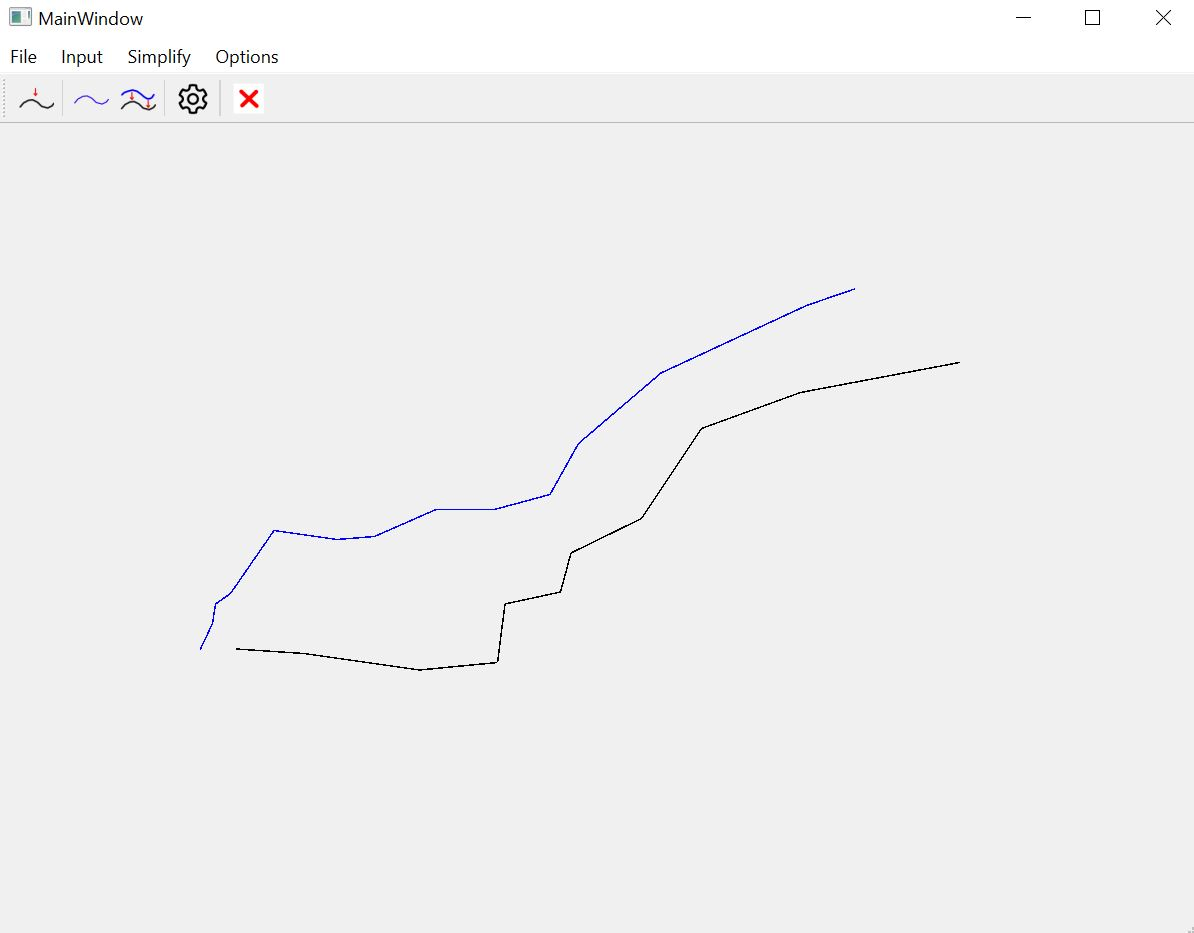
\includegraphics[width=12cm, height=10cm]{non_cross.JPG}
    \centering
    \caption{Ukázka aplikace se vstupními liniemi bez překřížení, zdroj: autoři.}
    \label{fig:obr1}
    \end{figure}
    
    \begin{figure}[htbp]
    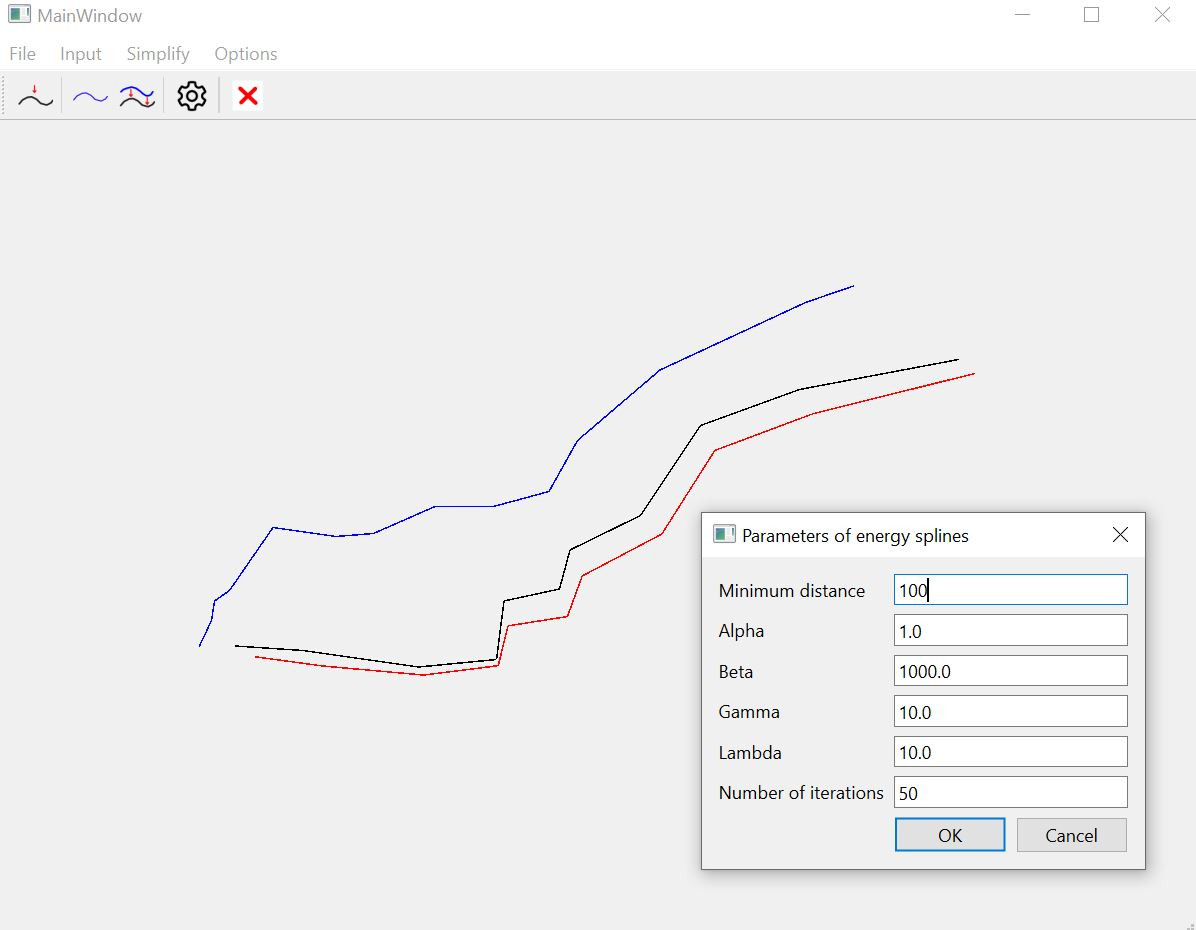
\includegraphics[width=12cm, height=10cm]{result_1.JPG}
    \centering
    \caption{Výsledné odsazení (červeně) při spuštění programu, zdroj: autoři.}
    \label{fig:obr1}
    \end{figure}
    
    \begin{figure}[htbp]
    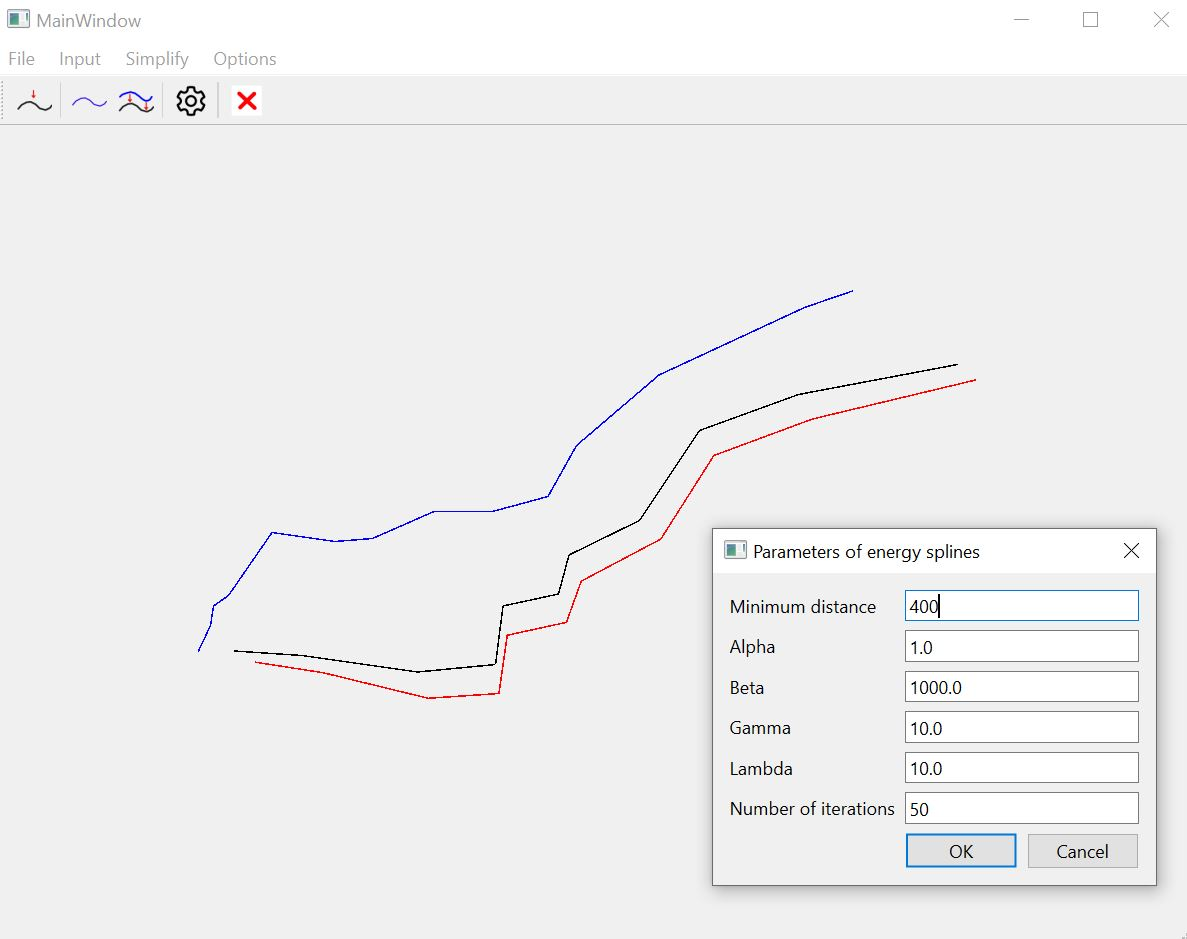
\includegraphics[width=12cm, height=10cm]{result_2.JPG}
    \centering
    \caption{Výsledné odsazení (červeně) při zvýšení minimální vzdálenosti, zdroj: autoři.}
    \label{fig:obr1}
    \end{figure}

    \begin{figure}[htbp]
    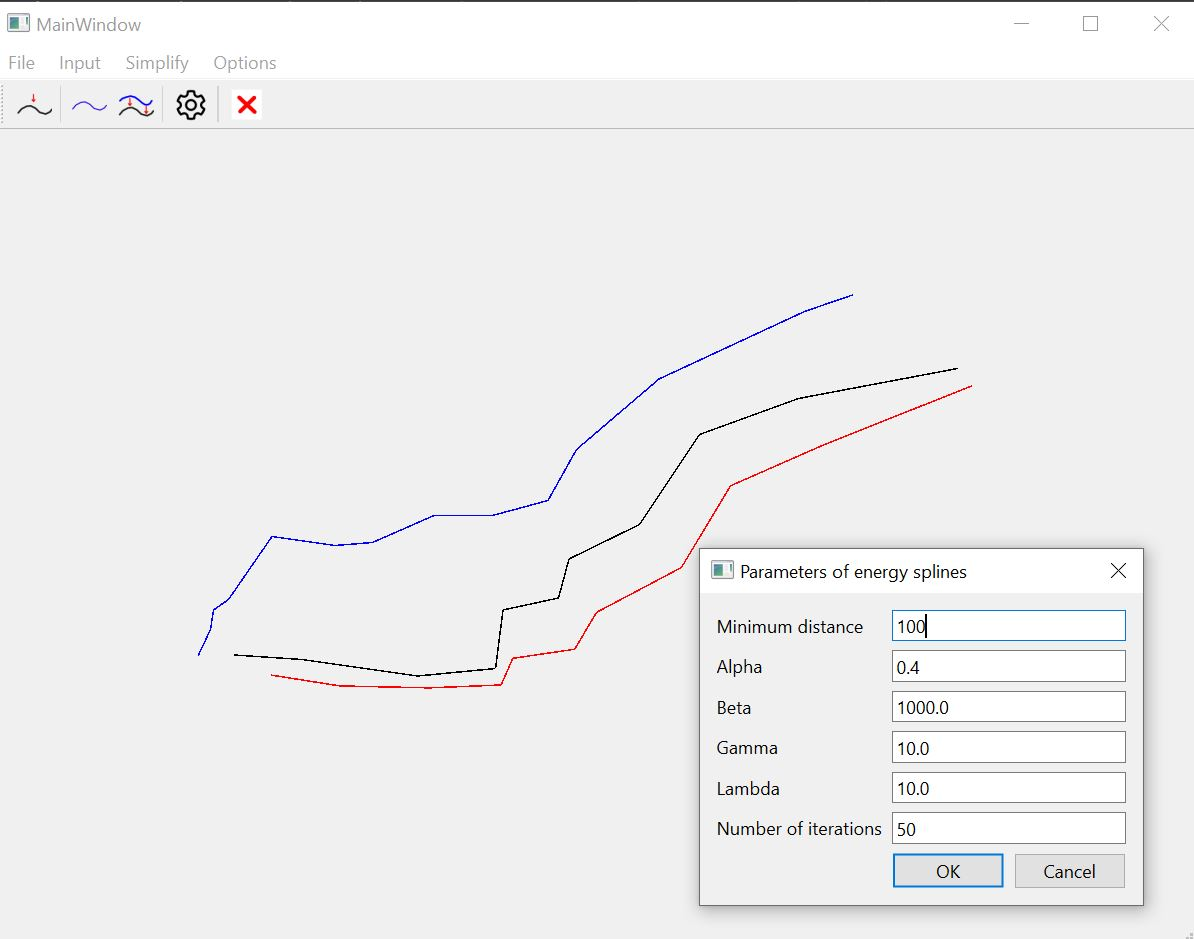
\includegraphics[width=12cm, height=10cm]{result_3.JPG}
    \centering
    \caption{Výsledné odsazení (červeně) při snížení paramteru Alfa, zdroj: autoři.}
    \label{fig:obr1}
    \end{figure}
    
    \begin{figure}[htbp]
    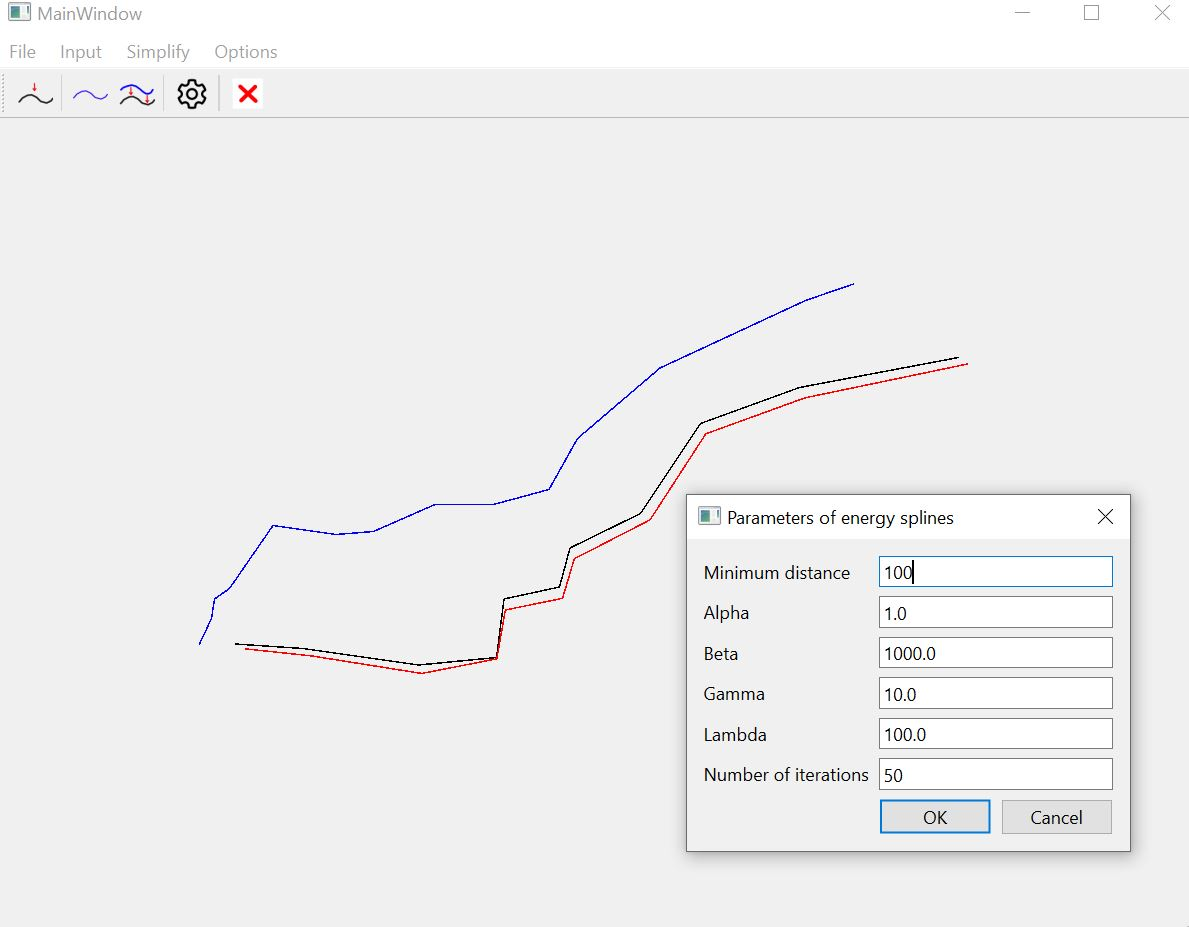
\includegraphics[width=12cm, height=10cm]{result_4.JPG}
    \centering
    \caption{Výsledné odsazení (červeně) při zvýšení parametru Lambda zdroj: autoři.}
    \label{fig:obr1}
    \end{figure}

    
    \newpage
    \section{Dokumentace}
        Aplikace je tvořena osmi skripty. Uživatelské rozhraní je tvořeno skriptem {\textit{mainform.py}}, jehož základ byl vytvořen pomocí softwaru QT Creator. Vizualizaci a vykreslování objektů zajišťuje skript {\textit{draw.py}}. Skript {\textit{algorithms.py}} definuje matematické metody pro správné provedení zvolených analýz. Skript {\textit{QPoint3DF}} definuje třídu QPoint3DF, která reprezentuje bod v 3D prostoru pomocí tří souřadnic (x, y, z). Skript {\textit{edge.py}} definuje třídu Edge pro reprezentaci hrany mezi dvěma body v trojrozměrném prostoru pomocí třídy QPoint3DF a implementuje několik metod pro práci s touto třídou, jako jsou získání počátečního a koncového bodu, vytvoření nové hrany s opačnou orientací a porovnání dvou hran. Skript {\textit{setting.py}} definuje dialogové okno pro nastavení parametrů energetických splinů. {\textit{mainwindow.py}} slouží k vytvoření uživatelského rozhraní aplikace. {\textit{triangle.py}} slouží k počítání sklonu a orientace trojúhelníku.
        
    \textbf{Metody skriptu \emph{mainform.py} :}
    \begin{itemize}
        \item \textbf{setupUi}: inicializuje a nastavuje různé prvky uživatelského rozhraní, jako např. velikost okna, hlavní widget, menu, lištu nástrojů a akce (např. otevření souboru, ukončení aplikace, vykreslení polygonu, analýza pozice bodů a polygonů apod.).
        
        \item \textbf{retranslateUi}: nastavení textů pro různé prvky uživatelského rozhraní.

        \item \textbf{settings}: Zobrazuje dialogové okno, které umožňuje uživateli nastavit parametry energiových splinů. Po potvrzení změn se získají hodnoty z dialogového okna a uloží se do příslušných proměnných.
        
        \item \textbf{inputL a inputB}: jsou volány při kliknutí na položky menu "Element" a "Barrier". Tyto metody slouží k nastavení cesty v závislosti na zvolené položce.

        \item \textbf{displaceClick}:  provádí posunutí jednoho prvku. Nejprve se získají souřadnice prvku a bariéry. Poté se používá algoritmus pro výpočet minimální energie spline.

        \item \textbf{drawLineClick}: slouží k aktivaci kreslení elementu.

        \item \textbf{drawBarrierClick}: slouží k aktivaci kreslení bariéry.

        \item \textbf{clearClick}: slouží k vymazání všech elementů a bariér.

        \item \textbf{exit}: ukočuje celou aplikaci.
        
    \end{itemize}

    \textbf{Metody skriptu \emph{algorithms.py} :}
    \begin{itemize}
        \item \textbf{getEuclidDistance}: vypočítá euklidovskou vzdálenost mezi dvěma body ($x_1, y_1$) a ($x_2, y_2$). Vrací vypočtenou vzdálenost.

        \item \textbf{getPointLineDistance}: vypočítá vzdálenost mezi bodem A $[x_a, y_a]$ a přímkou $(p_1, p_2)$. Nejprve se vypočítá hodnota $d_n$ a $d_d$ pomocí metody $getEuclidDistance$. Poté se vypočítává hodnota $d_1$ a $k$. Nakonec se vypočítávají souřadnice bodu na přímce $(x_q, y_q)$ nejbližšího bodu $A$ na přímce $(p_1, p_2)$. Metoda vrací hodnoty $d$ (vzdálenost bodu $A$ od přímky) a souřadnice $x_q, y_q$.

        \item \textbf{getPointLineSegmentDistance}: vypočítá vzdálenost mezi bodem $A [x_a, y_a]$a úsečkou $(p_1, p_2)$. Nejprve se vypočítávají hodnoty souřadnic bodů $P_3 a P_4$. Poté se pomocí metody getPointLineDistance vypočítávají hodnoty $d_13, xq_3, yq_3, d_24, xq_4, yq_4$. Dále se testuje podmínka $t$, a pokud platí, vrací se hodnoty vypočtené pomocí metody getPointLineDistance pro přímku $(p_1, p_2)$. Pokud neplatí, testují se podmínky $d_13$ a vrací se hodnoty vypočtené pomocí metody $getEuclidDistance$ pro body $p_1$ a $p_2$.
        
        \item \textbf{getNearestLineSegmentPoint}: hledá na překážce bod nejblíže bodu $A$. Nejprve se inicializují proměnné $imin$ a $dmin$. Poté se vypočítává vzdálenost $d_i$ a souřadnice $x_i$, $y_i$ pro každou úsečku na překážce. Pokud je vzdálenost $d_i$ menší než aktuální minimum $dmin$, aktualizuje se minimum a uloží se index úsečky a souřadnice nejbližšího bodu. Nakonec se vrací hodnoty $dmin$, $imin$, $xmin$, $ymin$.

        \item \textbf{createA}: vytváří matici A pro počítání energie. Nejprve se vypočítávají koeficienty $a, b, c$. Poté se vytvoří matice $A$ a nastavují se hodnoty pro hlavní diagonálu a další diagonály.

        \item \textbf{getEx}: vypočítá parciální derivaci vnější energie podle $x$. Nejprve se vypočítává hodnota $c$. Pokud je vzdálenost $d$ menší než $dmin$, vrací se hodnota parciální derivace. Jinak se vrací 0.

        \item \textbf{getEy}: vypočítá parciální derivaci vnější energie podle $y$. Nejprve se vypočítává hodnota $c$. Pokud je vzdálenost $d$ menší než $dmin$, vrací se hodnota parciální derivace. Jinak se vrací 0.

        \item \textbf{minEnergy}:  implementuje algoritmus pro výpočet minimální energie splinu. Nejprve se vytváří matice pro reprezentaci polylinie a překážky. Poté se vypočítává velikost kroku $h$. Následně se vytváří matice $A$ pomocí metody $createA$ a vypočítává se inverze matice $A$. Dále se vytvářejí matice pro rozdíly. Iterační proces probíhá v cyklu, ve kterém se vypočítávají parciální derivace potenciálu a posuny bodů. Nakonec se výsledná polylinie převede z matice na seznam bodů a vrátí se jako výstup.
        
    \end{itemize}

    \textbf{Metody skriptu \emph{edge.py} :}
    \begin{itemize}
    \item \textbf{getStart}: metoda, která vrací počáteční bod hrany.
    \item \textbf{getEnd}: metoda, která vrací koncový bod hrany.
    \item \textbf{switchOrientation}: metoda, která vytvoří novou hranu s opačnou orientací, tedy vymění počáteční a koncový bod.
    \item \textbf{eq}: metoda, která porovnává dvě hrany a vrací True, pokud jsou stejné (mají stejný počáteční a koncový bod), jinak vrací False
    \end{itemize}

    \textbf{Metody skriptu \emph{QPoint3DF.py} :}
    \begin{itemize}
    \item \textbf{getZ}: Metoda, která vrací hodnotu souřadnice z objektu QPoint3DF.
    \end{itemize}

    \textbf{Metody skriptu \emph{triangle.py} :}
    \begin{itemize}
    \item \textbf{getP1}: vrátí první vrchol trojúhelníku.
    \item \textbf{getP2}: vrátí druhý vrchol trojúhelníku.
    \item \textbf{getP3}: vrátí třetí vrchol trojúhelníku.
    \item \textbf{getSlope}: vrátí sklon trojúhelníku.
    \item \textbf{getAspect}: vrátí orientaci trojúhelníku.
    \end{itemize}

    \textbf{Metody skriptu \emph{mainwindow.py} :}
    \begin{itemize}
    \item \textbf{loadui}: načtení uživatelského rozhraní ze souboru form.ui a jeho zobrazení v okně aplikace.
    \end{itemize}

    \textbf{Metody skriptu \emph{draw.py} :}
    \begin{itemize}
    \item \textbf{setPath}:  slouží k načtení datového souboru pomocí dialogového okna. Přijímá parametry width a height, které určují rozměry okna. Dále určuje, zda se mají načíst body pro $L$ (False) nebo $B$ (True). Metoda umožňuje uživateli vybrat soubor pomocí dialogového okna a načte souřadnice bodů z vybraného souboru. Následně přepočítá souřadnice bodů tak, aby se vešly do okna aplikace. Načtené body jsou uloženy v příslušném polygonu.

    \item \textbf{switchSource}: sloužík přepnutí mezi pohybem bodu a přidáváním vrcholů.

    \item \textbf{getL}: metoda pro získání polygonu L.

    \item \textbf{getL}: metoda pro získání polygonu B. 

    \item \textbf{setLD}: metoda pro nastavení polygonu LD.

    \item \textbf{setSource}: metoda pro nastavení zdroje bodů. Přijímá parametr status, který určuje, zda jsou body přidávány do polygonu $L$ (True) nebo do polygonu $B$ (False). 
    
    \item \textbf{clearAll}: metoda pro vymazání všech polygonů. 
    

    \end{itemize}


    \section{Závěr}
    V tomto úkolu byla vytvořena aplikace využívající generalizační operátor Partial Modification. Ten umožňuje provést odsun a částečnou změnu jednoho blízkého prvku vzhledem k bariéře, aby nedocházelo k jejich grafickému konfliktu. Uživatel má možnost aplikovat tuto metodu na svá data, která načte do aplikace. Součástí aplikace je také možnost nastavit hodnoty parametrů pro tvorbu energetických splineů. V současné verzi aplikace je partial modification dostupná pouze pro jeden prvek a překážku. 

    Aplikace je bohužel funkční pouze částečně. Dochází k pádu programu při vstupních dat, které obsahují vzájemně se křížící linie. V případě nekřížících se linií je však odsun linie proveden správně a různá změna parametrů vytváří různé výsledky odsunu. Jako další možné vylepšení programu lze spatřovat v opravě programu, aby dokázal zpracovat i křížící se linie. Dalším vylepšením může být také možnost načítat mnohem více vstupních dat a provádět několik odsunů najednou.



    \newpage
    \section{Zdroje}
    Přednášky z předmětu \emph{Algoritmy z počítačové kartografie.}\\   

\end{document}
